\documentclass[10pt,journal]{IEEEtran}

\usepackage{cite}

\usepackage{tikz}
\usetikzlibrary{
  arrows.meta,
  positioning,
  fit,
  backgrounds
}
\usepackage{pgfplots}
\pgfplotsset{compat=1.18}
\usepackage{kotex}
\usepackage{amsmath,amssymb}
\usepackage{booktabs,graphicx,multirow,url}
\usepackage[hidelinks]{hyperref}

\interdisplaylinepenalty=2500
\setcounter{secnumdepth}{2}

\newcommand{\E}{\mathbb{E}}
\newcommand{\R}{\mathbb{R}}
\newcommand{\A}{\mathcal{A}}
\newcommand{\Sset}{\mathcal{S}}
\newcommand{\Dset}{\mathcal{D}}
\newcommand{\Qhard}{Q^{\mathrm{hard}}}
\newcommand{\Qmulti}{\widetilde{Q}}

\begin{document}

\title{Native Hybrid-Action Actor--Critic Learning\\
under Combinatorial Action Growth}

\author{Anonymous Authors}

\markboth{IEEE Transactions on Neural Networks and Learning Systems}%
{Anonymous Authors: Native Hybrid-Action Actor--Critic Learning under Combinatorial Action Growth}

\maketitle


\begin{abstract}
연속 제어와 복수의 이진 결정을 동시에 다루는 하이브리드 강화학습에서는 이진 변수의 수 $b$에 따라 결합 행동공간이 $2^b$으로 증가한다. 이때 모든 조합을 범주형 행동으로 열거하면 정책과 가치평가 비용이 빠르게 커지고, 각 이진 결정을 독립적으로 처리하면 행동 간 상호작용을 놓칠 수 있다. 본 연구는 이진 차원이 증가할 때 정책성능과 계산비용이 어떻게 변화하는지를 중심으로, 전체 결합행동을 열거하지 않는 native hybrid-action actor--critic을 제안한다.

제안 방법은 연속 행동과 이진 행동을 직접 생성하고, 실제 실행된 hard action으로 학습하는 pairwise structured twin critic을 사용한다. 각 critic의 Bernoulli 기대값은 해석적으로 계산할 수 있지만, actor가 사용하는 점별 clipped-twin value는 일반적으로 같은 이차 함수족에 속하지 않는다. 제안한 정책 갱신은 이 clipped objective 자체를 대상으로 하며, 상태 조건부 ANOVA control variate와 중요도 가중 잔차 보정을 결합하여 $2^b$개 행동을 열거하지 않고 가치와 기울기를 추정한다.

HardMove에서 결합 행동 수가 16개에서 1,024개로 증가하는 동안 제안 방법의 평균 성공률은 $0.534$--$0.630$ 범위를 유지하였다. 같은 구간에서 범주형 또는 파라미터화 기준선 중 여러 방법은 큰 성능저하를 보였고, HyAR는 작은 조건에서 더 높은 평균을 기록했지만 HM10에서 감소하였다. 가장 큰 HM10에서 제안 방법의 평균 학습시간은 HyAR보다 약 35\% 짧았다. 추가 환경은 다른 전이 및 보상구조에서의 적용성과 실행비용을 보완적으로 평가한다. 결과는 모든 조건에서의 절대적 우위가 아니라, 평가범위에서 조합 수 증가에 따른 성능 붕괴를 줄이면서 전체 열거와 잠재 행동 디코딩을 피하는 성능--비용 특성을 보여준다.
\end{abstract}

\begin{IEEEkeywords}
hybrid-action reinforcement learning, combinatorial action spaces,
multilinear value estimation, neural actor--critic, control variates.
\end{IEEEkeywords}

\IEEEpeerreviewmaketitle


\section{Introduction}
\label{sec:introduction}

강화학습은 일반적으로 유한한 이산 행동집합 또는 연속 벡터로 표현되는 행동공간을 가정한다. 보다 일반적인 순차적 의사결정 문제에서는 연속적인 제어량과 복수의 이진 결정이 하나의 시점에서 동시에 선택될 수 있다. 본 연구는 이러한 하이브리드 행동을
\begin{equation}
a=(a^c,a^d),\qquad
a^c\in\A^c\subseteq\R^m,\qquad
a^d\in\{-1,+1\}^b
\label{eq:hybrid-action}
\end{equation}
로 정의한다. 여기서 $a^c$는 연속 행동이고, $a^d$는 동시에 실행되는 $b$개의 이진 결정이다.

이 행동공간에서는 가능한 이진 조합의 수가 $2^b$으로 증가한다. 모든 조합을 하나의 범주형 행동으로 표현하면 정책과 가치함수의 출력 크기가 지수적으로 증가한다. 반대로 이진 행동을 독립적으로 처리하면 각 결정의 효과가 다른 이진 결정이나 연속 행동에 따라 달라지는 상호작용을 충분히 반영하기 어렵다.

파라미터화 행동 강화학습은 이산 행동과 해당 행동에 종속된 연속 파라미터를 함께 학습하는 방법을 제시하였다~\cite{masson2016,xiong2018,bester2019}. Hybrid Actor--Critic은 이산 선택과 연속 하위 정책을 결합하였으며~\cite{fan2019}, HyAR는 이산--연속 행동을 학습된 잠재공간으로 변환하였다~\cite{li2022hyar}. 이러한 방법은 주로 하나의 이산 선택과 그에 연결된 연속 파라미터를 대상으로 한다. 여러 이진 결정이 동시에 실행되는 경우에는 가능한 결합 행동과 행동 사이의 상호작용이 함께 증가한다.

대규모 이산 행동공간을 위한 행동 임베딩과 행동 분기 구조도 제안되었다~\cite{dulacarnold2015,tavakoli2018}. 행동 분기는 전체 조합을 열거하지 않고 차원별 값을 출력하여 계산량을 줄인다. 본 연구에서는 각 행동차원의 독립적인 가치만을 출력하지 않고, 주효과와 행동쌍 상호작용을 포함하는 결합 크리틱을 사용한다.

이산 행동을 연속적으로 이완하면 신경망을 통한 미분 가능한 정책학습이 가능하다~\cite{jang2017,maddison2017}. 환경에서 실행되는 행동은 이진값인 반면 정책 최적화에 사용되는 변수는 연속값이다. 이에 따라 실제 이진 행동에서 학습된 가치와 이완 공간에서 사용되는 정책 기울기를 일관된 원리로 연결하는 가치확장이 필요하다. 실제 이진 행동의 가치를 정확하게 평균하는 직접적인 방법은 모든 $2^b$개 조합을 평가해야 하므로 행동 차원이 증가할수록 계산량이 빠르게 증가한다.

본 연구의 중심 질문은 결합 행동 수가 지수적으로 증가할 때 전체 열거 없이 상호작용을 유지하고, 성능과 계산비용의 급격한 악화를 함께 줄일 수 있는가이다. 이를 위해 연속 행동과 $b$개의 이진 행동을 직접 생성하는 native actor, 주효과와 쌍대 상호작용을 갖는 hard-action twin critic, 그리고 제한된 질의예산에서 작동하는 다중선형 정책 갱신을 하나의 구조로 결합한다.

실제 실행 행동으로 학습된 critic은 Bernoulli 다중선형 확장을 통해 이완 정책변수와 연결된다. 핵심 계산문제는 개별 구조화 critic의 기대값이 아니라
\begin{equation}
\begin{aligned}
&\E_{Z\sim\mu_S}\!\left[\min_j Q_{\phi_j}^{\mathrm{hard}}(s,a^c,Z)\right]\\
&\qquad\neq
\min_j\E_{Z\sim\mu_S}\!\left[Q_{\phi_j}^{\mathrm{hard}}(s,a^c,Z)\right]
\end{aligned}
\label{eq:intro-clipped-gap}
\end{equation}
라는 clipped-objective mismatch이다. 점별 최솟값은 일반적으로 원래 pairwise quadratic class에 닫혀 있지 않다. 본 방법은 제한된 이진 질의로 이 점별 clipped value의 저차 구조를 amortize하고, 설명되지 않은 잔차를 importance-weighted score term으로 보정한다. 따라서 actor가 사용하는 목적을 개별 critic 기대값의 최솟값으로 바꾸지 않으면서 전체 $2^b$개 평가를 피한다.

본 연구의 주요 기여는 다음과 같다.

\begin{itemize}
    \item 전체 결합행동을 범주형으로 열거하지 않고 연속 제어와 복수의 이진 결정을 직접 생성하며, 실제 실행 행동의 pairwise interaction을 twin critic에 포함하는 native hybrid actor--critic을 제시한다.

    \item 실제 실행 행동의 점별 clipped-twin objective를 Bernoulli 다중선형 확장으로 정책변수와 연결하고, amortized low-order value와 importance-weighted residual correction을 결합한 bounded-query policy update를 구성한다. 꼭짓점 일치성과 조건부 가치차는 hard-action value와 이 갱신의 관계를 명시한다.

    \item 동일한 환경구조에서 결합 행동 수를 16개에서 1,024개로 증가시키고, 추가 환경에서도 단일 조건의 최고 평균이 아니라 성능 유지 양상, 학습시간 및 실행비용을 함께 평가한다.
\end{itemize}


\section{Related Work}
\label{sec:related-work}

\subsection{Parameterized and Hybrid Action Reinforcement Learning}

파라미터화 행동공간은 이산 행동과 각 이산 행동에 대응하는 연속 파라미터로 구성된다. Q-PAMDP는 이산 행동 선택과 연속 파라미터 정책을 교대로 최적화하였고~\cite{masson2016}, P-DQN은 연속 파라미터 생성기와 이산 행동의 Q-network를 하나의 심층 강화학습 구조로 결합하였다~\cite{xiong2018}.

P-DQN에서는 특정 이산 행동의 가치가 선택되지 않은 다른 행동의 연속 파라미터에도 의존할 수 있다. MP-DQN은 행동별 다중 통과 평가를 이용하여 선택된 이산 행동에 대응하는 파라미터만 Q-network에서 활성화한다~\cite{bester2019}. 이러한 방법들은 이산 행동과 연속 파라미터의 대응관계를 학습하며, 하나의 이산 행동을 선택하고 그 행동에 부속된 연속 파라미터를 결정하는 구조에 초점을 둔다.

Hybrid Actor--Critic은 이산 정책과 행동별 연속 하위 액터를 결합한다~\cite{fan2019}. HyAR는 조건부 변분 오토인코더와 환경 동역학 예측을 이용해 하이브리드 행동을 연속 잠재공간으로 변환한다~\cite{li2022hyar}. 잠재표현은 큰 하이브리드 행동공간을 압축하고, 디코더를 통해 원래 행동공간의 이산--연속 행동을 생성한다.

본 연구는 복수의 이진 결정과 연속 행동이 동시에 실행되는 행동공간을 다룬다. 이진 조합을 하나의 범주형 인덱스나 학습된 잠재 행동으로 변환하지 않으며, 환경에서 실제로 실행된 이진 행동으로 크리틱을 학습한다.


\subsection{Large and Factored Discrete Action Spaces}

Wolpertinger 구조는 이산 행동을 연속공간에 임베딩하고, 정책이 생성한 원형 행동 주변의 후보를 근사 최근접 탐색으로 선택한다~\cite{dulacarnold2015}. 이를 통해 매우 큰 이산 행동집합에서 전체 행동을 직접 평가하지 않고 후보집합을 구성한다.

Branching Dueling Q-Network는 공유 상태표현 뒤에 행동 차원별 분기를 배치하여 다차원 이산 행동을 생성한다~\cite{tavakoli2018}. 출력 수는 전체 결합 행동 수가 아니라 행동 차원 수에 대해 선형적으로 증가한다.

최근 action-decomposed reinforcement learning은 factored discrete actions의 projected Q-functions와 그 불편성 조건을 intervention semantics로 분석하였다~\cite{lee2025}. 본 연구는 이와 달리 연속--다중이진 행동에서 실행된 전체 hard action의 twin critic을 학습하고, 점별 clipped value를 제한된 질의로 정책에 전달한다.

본 연구 역시 전체 행동 조합을 정책 출력으로 열거하지 않는다. 행동분기나 projected Q-functions와 달리, 크리틱은 상태와 연속 행동을 조건으로 절편, 이진 주효과 및 쌍대 상호작용을 하나의 실행행동 가치로 결합한다. 따라서 각 이진 결정을 직접 출력하는 표현상의 이점과, clipped hard-action value를 제한된 질의로 갱신하는 이점을 함께 제공한다.


\subsection{Continuous Relaxations and Multilinear Extensions}

Gumbel--Softmax와 Concrete 분포는 이산 표본추출의 연속 이완을 통해 재매개화 기울기를 사용할 수 있게 한다~\cite{jang2017,maddison2017}. 이러한 방법은 이산 정책을 연속적인 계산 그래프에 포함할 수 있도록 한다.

본 연구는 이완 공간에서 별도의 크리틱을 학습하는 대신, 실제 이진 행동에서 학습한 크리틱의 다중선형 보간을 사용한다. 이진 꼭짓점 사이의 값은 Bernoulli 분포에서 실행 가능한 행동들의 가치를 평균한 값으로 정의되며, 각 이완 변수의 기울기는 실제 이진 행동 사이의 조건부 가치차로 연결된다.

다중선형 확장은 집합함수를 연속 초입방체로 확장하기 위해 조합최적화에서 사용되어 왔다~\cite{calinescu2011}. 본 연구는 독립 Bernoulli 표본에 대한 기대값이라는 원리를 일반적인 이진 행동 크리틱에 적용하여 연속 정책변수와 연결한다.


\subsection{Binary Query Designs and Control Variates}

직교배열은 제한된 설계점에서 개별 요인의 수준과 저차 조합을 균형 있게 관측하기 위한 실험설계 방법이며, 무작위화된 직교배열은 Monte Carlo 적분에서 저차 성분을 균형 있게 표본화하는 데 사용될 수 있다~\cite{owen1992,owen1994}. 쌍대 회귀항을 함께 식별하려면 균형성뿐 아니라 해당 설계행렬의 rank와 조건수도 확인해야 한다.

제어변량은 기대값을 계산할 수 있는 보조함수를 이용해 Monte Carlo 추정오차를 줄인다. 표본으로 학습한 함수를 제어변량으로 사용하는 방법은 중요도 표본추출과 이산 입력공간에도 적용될 수 있다~\cite{tracey2016}.

본 연구에서는 rank와 조건수를 확인한 이진 질의로 amortized ANOVA network를 학습한다. 대리모형의 기대값은 해석적으로 계산하고, hard-action critic과 대리모형 사이의 근사잔차를 별도 표본으로 보정한다.

본 연구의 차별점은 개별 수학도구보다 그 계산경로에 있다. 파라미터화 또는 잠재 행동법과 달리 이진 결정을 직접 생성하고 디코더 없이 hard action을 평가하며, 독립 분기법과 달리 pairwise value interaction을 유지한다. 또한 저차 구조를 control variate로 재사용한다. 이를 clipped twin objective 아래 결합하여 정책표현, 가치평가 및 실행비용이 $2^b$개의 명시적 출력에 의존하지 않도록 한다.


\section{Proposed Method}
\label{sec:method}

\subsection{Problem Formulation}

상태공간 $\Sset$, 하이브리드 행동공간
\begin{equation}
\A=\A^c\times\{-1,+1\}^b,
\end{equation}
전이확률 $P$, 보상함수 $r$ 및 할인율
$\gamma\in[0,1)$로 구성된 Markov 의사결정 과정을 고려한다. 정책의 목적은
\begin{equation}
J(\theta,\psi)
=
\E_{\pi_{\theta,\psi}}
\left[
\sum_{t=0}^{\infty}\gamma^t r_t
\right]
\label{eq:rl-objective}
\end{equation}
를 최대화하는 것이다.

환경에는 실행 가능한 이진 행동
$a^d\in\{-1,+1\}^b$를 전달한다. 정책 갱신에서는
$S\in[-1,1]^b$인 이완 스핀을 사용한다. $S$는 각 이진 결정의 평균과 가치 보간 위치를 나타내는 내부 정책변수이다.


\subsection{Overall Architecture}

제안 방법은 하이브리드 액터, 상태 조건부 logit-adjustment module, 실제 이진 행동으로 학습하는 구조화 쌍둥이 크리틱 및 제한된 질의 기반 다중선형 가치추정기로 구성된다. 전체 구조는 Fig.~\ref{fig:overall-architecture}와 같다. 정책과 critic은 결합행동별 출력을 만들지 않으며, 상호작용 구조와 질의예산을 통해 증가하는 이진 차원을 처리한다.

정책은 상태 $s_t$로부터 연속 행동 $a_t^c$와 이완 스핀 $S_t$를 생성한다. 학습 중에는 $\mu_{S_t}$에서 표본화한 이진 행동을 환경에 전달하고, 평가 시에는 $a_t^d=\operatorname{sign}(S_t)$를 사용한다. 환경 전이는 replay buffer에 저장되며, 크리틱은 실제 실행 행동으로 학습된다.

정책 갱신에서는 조건수 제약 이진 질의로 amortized ANOVA network를 학습하고, 대리모형의 해석적 기대값과 중요도 가중 잔차 score를 결합한다.


\begin{figure*}[t]
\centering
\resizebox{0.96\textwidth}{!}{
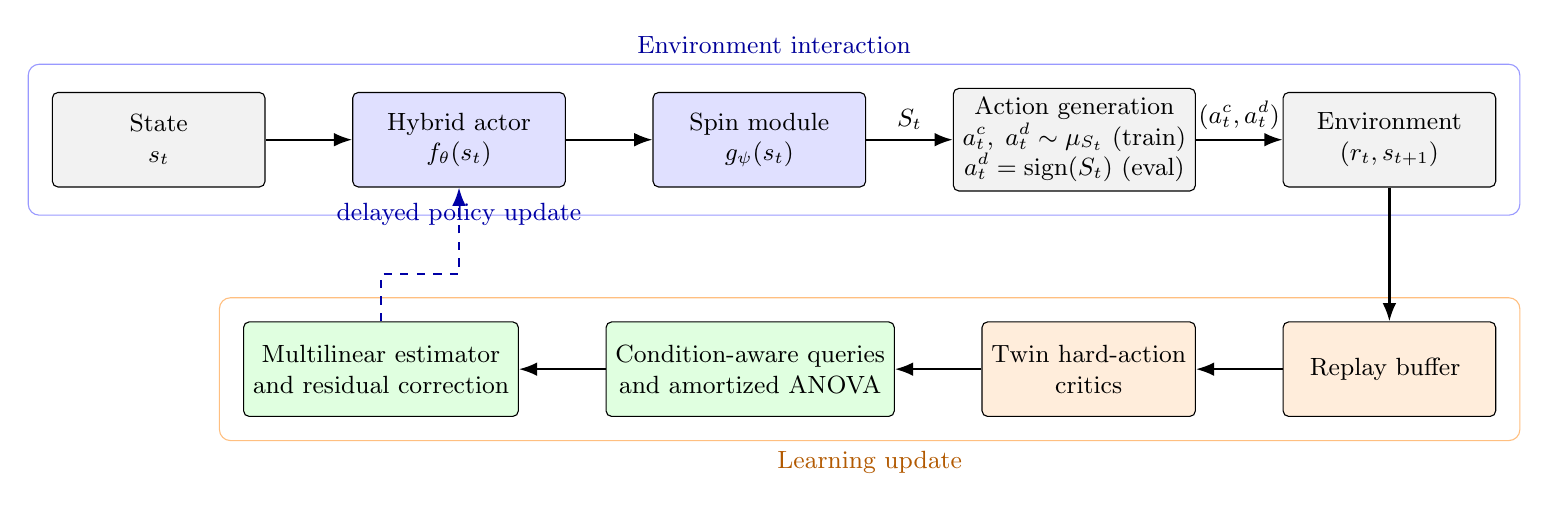
\begin{tikzpicture}[
    font=\small,
    >=Latex,
    node distance=8mm and 11mm,
    block/.style={
        draw,
        rounded corners=2pt,
        minimum width=27mm,
        minimum height=12mm,
        align=center,
        fill=gray!10
    },
    policy/.style={
        block,
        fill=blue!12
    },
    value/.style={
        block,
        fill=orange!14
    },
    estimator/.style={
        block,
        minimum width=34mm,
        fill=green!12
    },
    arrow/.style={
        ->,
        thick
    },
    update/.style={
        ->,
        thick,
        dashed,
        color=blue!65!black
    }
]

\node[block] (state) {State\\$s_t$};

\node[policy, right=of state] (actor) {
    Hybrid actor\\
    $f_\theta(s_t)$
};

\node[policy, right=of actor] (spin) {
    Spin module\\
    $g_\psi(s_t)$
};

\node[block, right=of spin] (action) {
    Action generation\\
    $a_t^c,\;a_t^d\sim\mu_{S_t}$ (train)\\
    $a_t^d=\operatorname{sign}(S_t)$ (eval)
};

\node[block, right=of action] (environment) {
    Environment\\
    $(r_t,s_{t+1})$
};

\node[value, below=17mm of environment] (replay) {
    Replay buffer
};

\node[value, left=of replay] (critic) {
    Twin hard-action\\
    critics
};

\node[estimator, left=of critic] (queries) {
    Condition-aware queries\\
    and amortized ANOVA
};

\node[estimator, left=of queries] (estimator) {
    Multilinear estimator\\
    and residual correction
};

\draw[arrow] (state) -- (actor);
\draw[arrow] (actor) -- (spin);
\draw[arrow] (spin) -- node[above] {$S_t$} (action);
\draw[arrow] (action) -- node[above] {$(a_t^c,a_t^d)$} (environment);
\draw[arrow] (environment) -- (replay);
\draw[arrow] (replay) -- (critic);
\draw[arrow] (critic) -- (queries);
\draw[arrow] (queries) -- (estimator);

\draw[update]
(estimator.north)
-- ++(0,6mm)
-| node[pos=0.72, above] {delayed policy update}
(actor.south);

\begin{scope}[on background layer]
\node[
    draw=blue!40,
    rounded corners=4pt,
    fit=(state)(actor)(spin)(action)(environment),
    inner sep=3mm,
    label={[blue!60!black]above:Environment interaction}
] {};

\node[
    draw=orange!50,
    rounded corners=4pt,
    fit=(replay)(critic)(queries)(estimator),
    inner sep=3mm,
    label={[orange!70!black]below:Learning update}
] {};
\end{scope}

\end{tikzpicture}
}
\caption{
Overall architecture of the proposed method.
Sampled training actions or deterministic evaluation actions are delivered
to the environment. Executed actions are stored in the replay buffer, and
the ANOVA control variate is used during policy learning.
}
\label{fig:overall-architecture}
\end{figure*}


\subsection{State-Conditioned Hybrid Policy}

하이브리드 액터 $f_\theta$는 상태로부터 연속 제어 로짓과 이진 제어 로짓을 생성한다.
\begin{equation}
(c_{\mathrm{ctrl}},b_{\mathrm{ctrl}})
=
f_\theta(s),
\label{eq:actor-output}
\end{equation}
여기서
$c_{\mathrm{ctrl}}\in\R^m$이고
$b_{\mathrm{ctrl}}\in\R^b$이다.

액터는 먼저 정규화된 연속 행동을
\begin{equation}
\bar a^c=\tanh(c_{\mathrm{ctrl}})\in(-1,1)^m
\label{eq:continuous-action}
\end{equation}
로 생성한다. 환경의 연속 행동범위가
$[a_{\min}^c,a_{\max}^c]$이면 성분별 affine 변환을 적용하여
$a^c=a_{\min}^c+(a_{\max}^c-a_{\min}^c)\odot(\bar a^c+\mathbf1)/2$로 전달한다.

구현에서 spin module이라 부르는 $g_\psi$는 이진 로짓을 상태에 따라 조정하기 위한 보조 logit-adjustment module이며, 상호작용행렬과 외부장을 출력한다.
\begin{equation}
(J_\psi(s),h_\psi(s))
=
g_\psi(s),
\label{eq:spin-module}
\end{equation}
여기서
$J_\psi(s)\in\R^{b\times b}$이고
$h_\psi(s)\in\R^b$이다. 상호작용행렬은 대칭화하고 대각성분을 0으로 설정한다. $J_\psi$는 다른 성분의 상태 조건부 field를 통해 각 Bernoulli 평균을 조정하지만, 식~\eqref{eq:training-action}의 조건부분포 자체에 확률적 상관을 도입하지는 않는다.

이완 스핀은
\begin{align}
\ell(s)
&=
h_\psi(s)
+
J_\psi(s)\tanh\!\left(h_\psi(s)\right)
+
b_{\mathrm{ctrl}},
\label{eq:effective-field}\\
S(s)
&=
\tanh\!\left(\ell(s)\right)
\in(-1,1)^b
\label{eq:relaxed-spin}
\end{align}
로 계산한다. 학습 중 환경 상호작용에서는 각 성분을
\begin{equation}
a_i^d\sim\operatorname{Bernoulli}_{\{-1,+1\}}
\!\left(\Pr(a_i^d=+1)=\frac{1+S_i}{2}\right)
\label{eq:training-action}
\end{equation}
에서 독립적으로 표본화한다. 평가 시에는 결정론적 행동
\begin{equation}
a_i^d
=
\begin{cases}
+1, & S_i\geq 0,\\
-1, & S_i<0
\end{cases}
\label{eq:executed-action}
\end{equation}
를 사용한다. 초기 warm-up 구간에서는 연속 행동과 이진 행동을 행동공간에서 무작위로 생성한다. 따라서 다중선형 목적은 warm-up 이후 학습 중 실제 사용되는 확률적 이진 정책의 기대가치와 직접 대응한다.


\subsection{Critic Learning on Executed Actions}

두 개의 크리틱
\begin{equation}
Q_{\phi_j}^{\mathrm{hard}}:
\Sset\times\A^c\times\{-1,+1\}^b
\rightarrow\R,
\qquad j\in\{1,2\},
\end{equation}
을 사용한다. 크리틱의 이진 입력은 이완 스핀이 아니라 replay buffer에 기록된 실제 실행 행동이다.

각 크리틱은 상태와 연속 행동의 공유 context로부터 절편, 주효과 및 모든 이진 행동쌍의 계수를 생성한다.
\begin{align}
Q_{\phi_j}^{\mathrm{hard}}(s,a^c,z)
&=q_{0,j}(s,a^c)
+\frac{1}{\sqrt b}\sum_{i=1}^{b}q_{i,j}(s,a^c)z_i
\nonumber\\
&\quad+\frac{1}{\sqrt{|\mathcal E_{\mathrm{all}}|}}
\sum_{(i,k)\in\mathcal E_{\mathrm{all}}}
q_{ik,j}(s,a^c)z_i z_k,
\label{eq:structured-critic}
\end{align}
여기서 $\mathcal E_{\mathrm{all}}=\{(i,k):1\leq i<k\leq b\}$이다. 이 구조는 각 성분을 독립적으로 평가하는 분기형 가치함수와 달리 쌍대 결합효과를 포함한다.

현재 정책이 결정론적으로 생성한 다음 행동을
$(a^{c\prime},a^{d\prime})$라 하면 TD target은
\begin{equation}
y
=
r+\gamma(1-d)
\min_{j\in\{1,2\}}
Q_{\phi_j'}^{\mathrm{hard}}
(s',a^{c\prime},a^{d\prime})
\label{eq:td-target}
\end{equation}
이다. 각 크리틱은
\begin{equation}
\mathcal{L}_{\mathrm{critic}}(\phi_j)
=
\E_{\Dset}
\left[
\left(
Q_{\phi_j}^{\mathrm{hard}}(s,a^c,a^d)-y
\right)^2
\right]
\label{eq:critic-loss}
\end{equation}
를 최소화한다. 쌍둥이 크리틱의 최솟값은 정책이 가치함수의 과대평가 오차를 활용하는 현상을 줄이기 위해 사용된다~\cite{fujimoto2018}.

다중선형 연산은 크리틱의 Bellman 학습 대상을 변경하지 않는다. 크리틱은 실제 이진 행동의 가치를 학습하고, 다중선형 확장은 정책 갱신 시 이 크리틱을 연속 변수 공간에서 사용하는 방법을 정의한다.

\subsection{Clipped-Twin Objective under Bounded Queries}

식~\eqref{eq:structured-critic}의 각 크리틱은 쌍대식이므로 독립 Bernoulli 분포에서 그 기대값을
\begin{align}
\widetilde Q_j(s,a^c,S)
&=q_{0,j}(s,a^c)
+\frac{1}{\sqrt b}\sum_i q_{i,j}(s,a^c)S_i
\nonumber\\
&\quad+\frac{1}{\sqrt{|\mathcal E_{\mathrm{all}}|}}
\sum_{(i,k)\in\mathcal E_{\mathrm{all}}}
q_{ik,j}(s,a^c)S_iS_k
\label{eq:analytic-single-critic}
\end{align}
로 정확히 계산할 수 있다. 그러나 actor가 사용하는 함수는
\begin{equation}
F_{\min}(z)=\min\{Q_{\phi_1}^{\mathrm{hard}}(s,a^c,z),
Q_{\phi_2}^{\mathrm{hard}}(s,a^c,z)\}
\label{eq:clipped-hard-value}
\end{equation}
이다. 각 크리틱이 이차식이더라도 $F_{\min}$은 일반적으로 원래 critic과 동일한 이차 형식을 유지하지 않으며,
\begin{equation}
\E_{\mu_S}[F_{\min}(Z)]
\neq
\min_j\widetilde Q_j(s,a^c,S)
\label{eq:min-expectation-gap}
\end{equation}
이다. 오른쪽 항을 사용하면 계산은 간단하지만 정책목적 자체가 바뀐다. 이후의 ANOVA--ACV 추정기는 개별 크리틱의 해석적 기대값을 근사하기 위한 것이 아니라, 왼쪽의 clipped twin objective를 유지하면서 그 기대값과 기울기를 제한된 hard-action 질의로 계산하기 위한 것이다.


\subsection{Multilinear Value Extension}

이완 스핀 $S\in[-1,1]^b$에 대해
\begin{equation}
\mu_S(z)
=
\prod_{i=1}^{b}
\frac{1+z_iS_i}{2},
\qquad
z\in\{-1,+1\}^b
\label{eq:bernoulli-measure}
\end{equation}
를 정의한다. 이 분포에서
\begin{equation}
\Pr(z_i=+1)=\frac{1+S_i}{2},
\qquad
\E_{\mu_S}[z_i]=S_i
\end{equation}
가 성립한다.

정책 갱신에 사용하는 clipped hard-action value의 다중선형 확장은
\begin{align}
\widetilde Q_{\min}(s,a^c,S)
&=
\E_{z\sim\mu_S}
\left[
Q_{\min}^{\mathrm{hard}}(s,a^c,z)
\right]
\nonumber\\
&=
\sum_{z\in\{-1,+1\}^b}
Q_{\min}^{\mathrm{hard}}(s,a^c,z)
\prod_{i=1}^{b}
\frac{1+z_iS_i}{2}
\label{eq:multilinear-extension}
\end{align}
로 정의한다. 식~\eqref{eq:multilinear-extension}은 실제 이진 행동에서 계산된 clipped twin value를 Bernoulli 기대연산을 통해 연속 변수 $S$와 연결한다. 다음의 꼭짓점 일치성과 조건부 가치차는 임의의 hard-action 함수에 성립하므로 $Q_{\min}^{\mathrm{hard}}$에도 그대로 적용된다.


\subsubsection{Vertex Consistency}

임의의 이진 꼭짓점
$v\in\{-1,+1\}^b$에서 $\mu_v$는 $z=v$에 모든 확률을 부여한다. 따라서
\begin{equation}
\widetilde Q_{\min}(s,a^c,v)
=
Q_{\min}^{\mathrm{hard}}(s,a^c,v)
\label{eq:vertex-consistency}
\end{equation}
가 성립한다. 즉, 연속 가치확장은 모든 실행 가능한 이진 행동에서 원래 크리틱과 정확히 일치한다.


\subsubsection{Conditional Value Difference}

$z_{-i}$를 $i$번째 성분을 제외한 이진 벡터라 하면,
\begin{align}
\frac{\partial\widetilde Q_{\min}}{\partial S_i}
&=
\frac{1}{2}
\E_{z_{-i}\sim\mu_{S_{-i}}}
\big[
Q_{\min}^{\mathrm{hard}}(s,a^c,+1,z_{-i})
\nonumber\\
&\hspace{28mm}
-
Q_{\min}^{\mathrm{hard}}(s,a^c,-1,z_{-i})
\big].
\label{eq:conditional-difference}
\end{align}

따라서 $S_i$에 대한 가치 기울기는 다른 행동들을 현재 정책분포에 따라 평균했을 때, $i$번째 이진 결정을 $-1$에서 $+1$로 전환하여 얻는 조건부 가치차의 절반이다. 이 관계를 통해 이완 공간의 기울기가 실제 이진 행동의 가치차에 의해 결정된다.


\subsection{Amortized Sparse ANOVA Control Variate}

식~\eqref{eq:multilinear-extension}의 정확한 계산에는 $2^b$개의 크리틱 질의가 필요하다. 이를 완화하기 위해 상태와 연속 행동으로부터 ANOVA 계수를 예측하는 amortized network를 사용한다. 대리모형은
\begin{equation}
g_\eta(z;s,a^c)
=
\beta_0
+
\sum_{i=1}^{b}\beta_i z_i
+
\sum_{(i,j)\in\mathcal{E}}
\beta_{ij}z_i z_j
\label{eq:anova-surrogate}
\end{equation}
형태이다. $\mathcal{E}$는 대리모형이 사용하는 $K$개의 이진 행동쌍이다. 네트워크는 절편, 모든 주효과 및 선택된 쌍대 계수를 출력한다. 모든 후보쌍의 예측계수 크기를 기준으로 상위 $K$개를 결정하며, 이 선택은 역전파 경로에서 분리한다.

ANOVA network는 제한된 이진 질의에서 얻은
$Q_{\min}^{\mathrm{hard}}$를 회귀목표로 학습한다. 질의 설계는
$p=1+b+K$개의 선택된 항에 대해 최소 $2p$개의 Rademacher 행을 생성하고,
$\operatorname{rank}(X_{\mathcal E})=p$ 및
$\kappa(X_{\mathcal E})\leq100$을 만족하지 않으면 행 수를 증가시킨다.
따라서 본 구현의 설계는 고전적인 strength-2 직교배열 자체가 아니라,
rank와 조건수를 명시적으로 검사하는 조건수 제약 이진 설계이다.
생성 절차와 진단량은 Supplement에 제시한다.

$\mu_S$에서 이진 변수들이 독립이므로
\begin{equation}
\E_{\mu_S}[z_i]=S_i,
\qquad
\E_{\mu_S}[z_iz_j]=S_iS_j
\end{equation}
가 성립한다. 따라서 대리모형의 기대값은
\begin{equation}
\widetilde g_\eta(S)
=
\beta_0
+
\sum_{i=1}^{b}\beta_iS_i
+
\sum_{(i,j)\in\mathcal{E}}
\beta_{ij}S_iS_j
\label{eq:anova-expectation}
\end{equation}
로 추가적인 크리틱 질의 없이 계산할 수 있다.

본 연구에서는 $g_\eta$를 최종 크리틱이 아닌 제어변량으로 사용한다. ANOVA network의 계수는 actor와 spin module을 갱신할 때 고정하며, hard-action critic과 amortized 예측값의 차이는 다음 절의 잔차항으로 보정한다.


\subsection{Importance-Weighted ACV Score Estimation}

목표 Bernoulli 분포와 균등분포 $u(z)=2^{-b}$를 결합한 proposal을
\begin{equation}
q_\epsilon(z\mid S)
=
(1-\epsilon)\mu_S(z)+\epsilon 2^{-b}
\label{eq:proposal-distribution}
\end{equation}
로 정의한다. 중요도 가중치는
\begin{equation}
w(z,S)
=
\frac{\mu_S(z)}{q_\epsilon(z\mid S)}
\label{eq:importance-weight}
\end{equation}
이다.

대리모형이 설명하지 못한 크리틱 잔차는
\begin{equation}
\delta_\phi(z)
=
Q_{\min}^{\mathrm{hard}}(s,a^c,z)-g_\eta(z)
\end{equation}
로 정의한다. 다중선형 가치 자체의 중요도 표본 추정기는
\begin{align}
\widehat Q_{\mathrm{ACV}}(s,a^c,S)
&=
\widetilde g_\eta(S)
\nonumber\\
&\quad+
\frac{1}{M}
\sum_{k=1}^{M}
    w(z^{(k)},S)\delta_\phi(z^{(k)}),
\label{eq:acv-estimator}\\
&\hspace{22mm}
    z^{(k)}\sim q_\epsilon(\cdot\mid S)
\nonumber
\end{align}
이다.

실제 이진 정책 갱신에서는 이 값 추정기를 그대로 자동미분하지 않고 score-function identity를 사용한다. $\eta$, $w$ 및 $\delta_\phi$를 해당 갱신에서 상수로 취급하면 사용되는 확률적 목적은
\begin{align}
\widehat{\mathcal J}_{d}(S)
&=
\widetilde g_\eta(S)
+\frac{1}{M}\sum_{k=1}^{M}
\operatorname{sg}\!\left(
w_k\delta_k
\right)
\log\mu_S(z^{(k)})
\label{eq:score-objective}
\end{align}
이다. 여기서 $w_k=w(z^{(k)},S)$와
$\delta_k=Q_{\min}^{\mathrm{hard}}(s,a^c,z^{(k)})-g_\eta(z^{(k)})$이며,
$\operatorname{sg}$는 역전파에서 기울기를 차단한다. 이 목적의 수치값 자체가
$\widetilde Q_{\min}$의 추정값인 것은 아니지만, 그 $S$-gradient는 중요도 가중 ACV
policy-gradient estimator가 된다. ANOVA 학습용 설계질의와 잔차 표본은 별도로 생성한다.


\subsection{Policy Objective and Training}

정책 갱신에서는 두 크리틱의 보수적인 값
\begin{equation}
Q_{\min}^{\mathrm{hard}}(s,a^c,z)
=
\min_{j\in\{1,2\}}
Q_{\phi_j}^{\mathrm{hard}}(s,a^c,z)
\end{equation}
을 사용한다. 각 크리틱은 식~\eqref{eq:structured-critic}의 이차 구조를 갖지만 두 함수의 점별 최솟값은 일반적으로 원래 critic과 동일한 이차 형식을 유지하지 않는다. 따라서 $Q_{\min}^{\mathrm{hard}}$의 Bernoulli 기대값에는 amortized surrogate와 잔차 보정을 적용한다. 이진 정책은 식~\eqref{eq:score-objective}로 갱신하고,
연속 정책은 평가 이진 행동
$a_{\mathrm{det}}^d=\operatorname{sign}(S)$에서의
$Q_{\min}^{\mathrm{hard}}(s,a^c,a_{\mathrm{det}}^d)$를 직접 미분하여 갱신한다.

이완 스핀이 이진 꼭짓점에 가까워지도록
\begin{equation}
\mathcal{R}_{\mathrm{bin}}(S)
=
\frac{1}{b}
\sum_{i=1}^{b}(1-S_i^2)^2
\label{eq:binary-regularizer}
\end{equation}
를 사용한다. 구현의 actor 및 spin 손실은
\begin{align}
\mathcal{L}_{\mathrm{actor}}(\theta,\psi)
&=\E_{s\sim\Dset}\!\Bigg[
\frac{1}{2m}\|c_{\mathrm{ctrl}}\|_2^2
+\lambda_{\mathrm{bin}}\mathcal R_{\mathrm{bin}}(S)
\nonumber\\
&\hspace{13mm}
-\frac{1}{\alpha}Q_{\min}^{\mathrm{hard}}
(s,a^c,a_{\mathrm{det}}^d)
-\frac{1}{\alpha}\widehat{\mathcal J}_{d}(S)
\Bigg]
\label{eq:actor-objective}
\end{align}
이다. $\alpha>0$는 가치항의 척도를 조절한다.

크리틱은 매 학습 단계에서 replay buffer의 실제 실행 행동으로 갱신한다. 정책 갱신 시에는 먼저 조건수 제약 설계질의로 ANOVA network를 갱신한 뒤, 별도의 mixture 표본으로 actor와 spin module을 갱신한다. actor와 spin module은 동일한 목적을 사용하되 서로의 파라미터를 고정한 교대 gradient step을 수행한다. 지연 정책 갱신과 Polyak averaging으로 갱신되는 target critic은 안정적인 가치학습을 위해 사용한다~\cite{fujimoto2018}. 전체 절차와 hyperparameter는 Supplement에 제시한다.


\subsection{Computational Complexity}

hard-action critic을 black-box로 평가하여 정확한 다중선형 합을 계산하면 상태 하나당 $2^b$회의 질의가 필요하다. 조건수 제약 설계의 질의 수를 $N_{\mathrm{des}}$, 잔차 표본 수를 $M$이라 하면 제안 방법의 질의점 수는
\begin{equation}
N_{\mathrm{query}}
=
N_{\mathrm{des}}+M
\label{eq:query-complexity}
\end{equation}
이다. 두 개의 크리틱을 모두 평가할 경우 실제 critic forward pass 수는 $2(N_{\mathrm{des}}+M)$이다.

모든 쌍대 항을 사용하면 ANOVA 모형은 $O(b^2)$개의 항을 갖는다. $K$개의 상호작용만 선택하면 대리모형의 항과 해석적 기대값 계산비용은 $O(b+K)$가 된다. 따라서 $N_{\mathrm{des}}$, $M$ 및 $K$를 제한하면 정책 갱신 비용이 전체 행동 조합 수에 직접 비례하지 않는다.

기본설정 $K=b$, $N_{\mathrm{des}}=2(1+b+K)$ 및 $M=2(1+b+K)$에서 첫 설계가 조건수 검사를 통과하면 $N_{\mathrm{query}}=4+8b$이다. 이에 따라 HM4, HM6, HM8 및 HM10의 질의점 수는 각각 36, 52, 68 및 84이고, 전체 열거의 16, 64, 256 및 1,024개와 비교된다. 따라서 제안 방식은 매우 작은 HM4에서 전체 열거보다 적은 질의를 사용하지 않는다. 본 방법의 계산상 목적은 모든 작은 문제에서 열거보다 저렴하다는 것이 아니라, 이진 차원이 증가할 때 질의 수가 $2^b$에 직접 비례하는 것을 피하는 데 있다.

이 비교에서 중요한 crossover는 기본설정의 estimator query-point 수가 $b$에 대해 선형적으로 증가하는 반면 전체 열거는 지수적으로 증가한다는 점이다. 이는 전체 알고리즘이 $O(b)$이라는 주장이 아니다. 작은 $b$에서는 정확한 다중선형 값을 기준으로 수치적 일관성을 확인하고, 차원이 증가하는 실험에서는 정책 성능의 유지 여부, 크리틱 질의 수 및 실제 계산시간을 함께 평가한다.
\section{Theoretical Properties}
\label{sec:theoretical-properties}

본 절은 전체 행동열거 없이 사용하는 정책 갱신이 어떤 hard-action 목적에 연결되는지를 정리한다. 앞의 두 성질은 알려진 다중선형 확장의 기본 결과이며, 실제 실행 행동에서 학습된 $Q_{\min}^{\mathrm{hard}}$와 이완 정책변수 사이의 관계를 명확히 한다. 이어지는 잔차 보정 결과는 제한된 질의로 이 목적의 gradient를 추정하는 본 구현의 정당성을 제공한다. 상세한 증명과 추가 유도는 Supplement에 제시한다.


\subsection{Uniqueness and Vertex Consistency}

\noindent\textbf{Proposition 1 (Vertex-consistent multilinear extension).}
고정된 상태 $s$와 연속 행동 $a^c$에 대해
\begin{equation}
F(S)
=
\sum_{z\in\{-1,+1\}^b}
Q_{\min}^{\mathrm{hard}}(s,a^c,z)
\prod_{i=1}^{b}\frac{1+z_iS_i}{2}
\label{eq:theory-extension}
\end{equation}
라 하자. 그러면 $F$는 각 $S_i$에 대해 일차인 다중선형 함수이며, 모든
$v\in\{-1,+1\}^b$에 대해
\begin{equation}
F(v)=Q_{\min}^{\mathrm{hard}}(s,a^c,v)
\label{eq:theory-vertex}
\end{equation}
를 만족한다. 또한 이러한 꼭짓점 조건을 만족하는 다중선형 함수는 유일하다.

\noindent\emph{Proof sketch.}
$S=v$인 경우 각 곱항은
\begin{equation}
\prod_{i=1}^{b}\frac{1+z_iv_i}{2}
=
\begin{cases}
1, & z=v,\\
0, & z\neq v
\end{cases}
\end{equation}
가 된다. 따라서 식~\eqref{eq:theory-extension}에서는 $z=v$에 대응하는 항만 남아 식~\eqref{eq:theory-vertex}를 얻는다. 각 곱항은 모든 $S_i$에 대해 일차이므로 $F$는 다중선형이다. $b$개 변수의 다중선형 함수는
\begin{equation}
F(S)=\sum_{U\subseteq\{1,\ldots,b\}}c_U\prod_{i\in U}S_i
\end{equation}
로 표현되며, $2^b$개의 계수 $c_U$는 $2^b$개 꼭짓점 값에 의해 유일하게 결정된다.

Proposition 1은 이완 공간의 가치가 임의의 외삽으로 정의되지 않고, 실제 이진 행동에서 학습한 크리틱 값에 의해 유일하게 결정됨을 의미한다.


\subsection{Gradient as a Conditional Action Advantage}

\noindent\textbf{Proposition 2 (Conditional binary value difference).}
$\widetilde Q_{\min}=F$라 하면 각 이완 변수 $S_i$에 대해
\begin{align}
\frac{\partial \widetilde Q_{\min}}{\partial S_i}
&=
\frac{1}{2}
\E_{z_{-i}\sim\mu_{S_{-i}}}
\Big[
Q_{\min}^{\mathrm{hard}}(s,a^c,+1,z_{-i})
\nonumber\\
&\hspace{27mm}
-
Q_{\min}^{\mathrm{hard}}(s,a^c,-1,z_{-i})
\Big].
\label{eq:theory-gradient}
\end{align}

\noindent\emph{Proof sketch.}
Bernoulli 측도를 $i$번째 성분과 나머지 성분으로 분리하면
\begin{align}
\widetilde Q_{\min}
&=
\frac{1+S_i}{2}
\E_{z_{-i}}
[Q_{\min}^{\mathrm{hard}}(s,a^c,+1,z_{-i})]
\nonumber\\
&\quad+
\frac{1-S_i}{2}
\E_{z_{-i}}
[Q_{\min}^{\mathrm{hard}}(s,a^c,-1,z_{-i})].
\end{align}
이를 $S_i$에 대해 미분하면 식~\eqref{eq:theory-gradient}를 얻는다.

식~\eqref{eq:theory-gradient}의 양수 방향은 다른 이진 행동을 현재 정책분포에 따라 평균했을 때 $a_i^d=+1$의 가치가 더 높음을 의미한다. 반대로 음수 방향은 $a_i^d=-1$의 조건부 가치가 더 높음을 의미한다. 따라서 다중선형 기울기는 각 이진 행동에 대한 상태 및 행동 조건부 advantage로 해석할 수 있다.


\subsection{Unbiased Residual Correction}

ANOVA 대리모형을 $g_\eta(z)$라 하고, 목표분포와 제안분포를 각각 $\mu_S(z)$와 $q_\epsilon(z\mid S)$라 하자. 다음의 지지집합 조건을 가정한다.
\begin{equation}
\mu_S(z)>0
\quad\Longrightarrow\quad
q_\epsilon(z\mid S)>0.
\label{eq:support-condition}
\end{equation}

\noindent\textbf{Proposition 3 (ACV expectation).}
고정된 대리모형 $g_\eta$와 독립적인 잔차 표본
$z^{(k)}\sim q_\epsilon(\cdot\mid S)$에 대해
\begin{align}
\widehat Q_{\mathrm{ACV}}
&=
\widetilde g_\eta(S)
+
\frac{1}{M}\sum_{k=1}^{M}
\frac{\mu_S(z^{(k)})}
{q_\epsilon(z^{(k)}\mid S)}
\nonumber\\
&\hspace{16mm}\times
\left[
Q_{\min}^{\mathrm{hard}}(s,a^c,z^{(k)})
-
g_\eta(z^{(k)})
\right]
\end{align}
라 하면
\begin{equation}
\E[
\widehat Q_{\mathrm{ACV}}
\mid g_\eta
]
=
\widetilde Q_{\min}(s,a^c,S)
\label{eq:acv-expectation-theory}
\end{equation}
가 성립한다.

\noindent\emph{Proof sketch.}
잔차를
$\delta_\phi(z)=Q_{\min}^{\mathrm{hard}}(s,a^c,z)-g_\eta(z)$라 하면,
\begin{align}
\E_{q_\epsilon(\cdot\mid S)}
\left[
\frac{\mu_S(z)}{q_\epsilon(z\mid S)}
\delta_\phi(z)
\right]
&=
\sum_z
q_\epsilon(z\mid S)
\frac{\mu_S(z)}{q_\epsilon(z\mid S)}
\delta_\phi(z)
\nonumber\\
&=
\E_{\mu_S}[\delta_\phi(z)].
\end{align}
또한
$\widetilde g_\eta(S)=\E_{\mu_S}[g_\eta(z)]$이므로 두 항을 더하면
$\E_{\mu_S}[Q_{\min}^{\mathrm{hard}}]$가 되어
식~\eqref{eq:acv-expectation-theory}를 얻는다.

이 성질은 amortized ANOVA 대리모형이 clipped twin value와 정확히 일치하지 않더라도 잔차 보정을 통해 그 다중선형 가치에 연결될 수 있음을 보여준다.

\noindent\textbf{Corollary 1 (Unbiased ACV score gradient).}
Proposition 3의 조건에서 $g_\eta$를 정책 갱신 동안 고정하고
\begin{align}
\widehat G_S
&=\nabla_S\widetilde g_\eta(S)
 +\frac{1}{M}\sum_{k=1}^{M}
 w(z^{(k)},S)\delta_\phi(z^{(k)})
 \nabla_S\log\mu_S(z^{(k)})
\label{eq:acv-gradient-theory}
\end{align}
라 하면
\begin{equation}
\E_{q_\epsilon}[\widehat G_S]
=\nabla_S\widetilde Q_{\min}(s,a^c,S)
\end{equation}
가 성립한다.

\noindent\emph{Proof sketch.}
$\nabla_S\E_{\mu_S}[\delta_\phi]
=\E_{\mu_S}[\delta_\phi\nabla_S\log\mu_S]$에 중요도 항등식을 적용하면
\begin{equation}
\E_{q_\epsilon}\!\left[
w\delta_\phi\nabla_S\log\mu_S
\right]
=\nabla_S\E_{\mu_S}[\delta_\phi]
\end{equation}
을 얻는다. 여기에 $\nabla_S\widetilde g_\eta$를 더하면 결과가 성립한다.
구현에서는 $w\delta_\phi$를 detach한 식~\eqref{eq:score-objective}의
자동미분으로 동일한 추정량을 계산한다.


\subsection{Query Complexity}

\noindent\textbf{Corollary 2 (Budgeted critic queries).}
정확한 black-box 다중선형 합은 상태와 연속 행동 하나당 $2^b$회의 hard critic 질의를 요구한다. 제안 방법에서 설계질의 수가 $N_{\mathrm{des}}$이고 잔차 표본 수가 $M$이면 정책 갱신당 질의점 수는
\begin{equation}
N_{\mathrm{query}}
=
N_{\mathrm{des}}+M
\end{equation}
이다. 또한 $K$개의 쌍대 항을 사용하는 희소 ANOVA의 해석적 기대값은
\begin{equation}
O(b+K)
\end{equation}
의 연산으로 계산된다.

따라서 $N_{\mathrm{des}}$, $M$ 및 $K$를 고정하거나 행동 차원에 대해 다항적으로 증가시키면, 정책 갱신은 $2^b$개의 전체 행동 조합을 직접 열거하지 않고 수행된다. Proposition 1--3과 Corollary 1은 이진 꼭짓점의 가치 일관성, 조건부 가치차, 잔차 보정의 기대값 및 score-function 정책기울기의 기대값을 각각 정리한다.

\section{Experimental Evaluation}
\label{sec:experiments}

\subsection{Environments and Evaluation Protocol}

Table~\ref{tab:experiment-overview}은 평가환경과 각 환경에서 사용하는 행동 차원, 학습 예산 및 평가 목적을 요약한다.

\begin{table}[t]
\centering
\caption{Summary of the experimental environments.}
\label{tab:experiment-overview}
\resizebox{\columnwidth}{!}{
\begin{tabular}{lcccc}
\toprule
Environment & Binary dim. & Combinations & Interactions & Evaluation role\\
\midrule
HardMove-4  & 4  & 16    & 1M   & Controlled scaling\\
HardMove-6  & 6  & 64    & 1M   & Controlled scaling\\
HardMove-8  & 8  & 256   & 1M   & Controlled scaling\\
HardMove-10 & 10 & 1,024 & 1M   & Controlled scaling\\
Cogen-BC    & 6  & 64    & 500k & Additional environment\\
GymInvMgmt-C6  & 6  & 64    & 500k & Cross-domain scaling\\
GymInvMgmt-C8  & 8  & 256   & 500k & Cross-domain scaling\\
GymInvMgmt-C10 & 10 & 1,024 & 500k & Cross-domain scaling\\
\bottomrule
\end{tabular}
}
\end{table}

HardMove는 연속 이동량과 복수의 이진 결정을 동시에 포함하는 통제된 환경이다. HM4, HM6, HM8 및 HM10은 환경의 기본 구조와 보상체계를 유지하면서 이진 행동 차원만 증가시킨다. 이를 통해 결합 행동 수가 16개에서 1,024개로 증가할 때의 정책 성능과 계산비용을 직접 평가한다.

Cogen-BC는 SustainGym Cogen~\cite{yeh2023}의 전이 및 보상구조를 바탕으로 여섯 개의 이진 행동과 여덟 개의 연속 행동을 정책이 함께 결정하도록 구성한 환경이다. Cogen-BC에서는 행동 차원을 변화시키지 않고 하나의 고정된 설정에서 비교 방법들과의 제어 성능을 평가한다. 큰 관측값과 보상척도를 안정적으로 처리하기 위해 제안 방법의 critic에는 관측 표준화와 PopArt형 Q 정규화를 적용하였으며, 구체적인 절차는 Supplement에 제시한다.

GymInvMgmt에서는 동일한 10단계 네트워크 구조에서 정책이 제어하는 행동 마스크를 변경하여 C6, C8 및 C10 조건을 구성한다. 따라서 GymInvMgmt는 HardMove와 다른 상태전이 및 보상구조에서 이진 행동 차원이 6, 8, 10으로 증가할 때의 성능 변화를 평가하는 교차환경 확장성 실험으로 사용한다.

모든 주요 결과는 다섯 개의 독립적인 training seed로 평가한다. 각 표의 평균과 표준편차는 training seed를 기준으로 계산한다.


\subsection{Baselines and Metrics}

HardMove에서는 HyAR-TD3~\cite{li2022hyar}, PDQN-TD3, PA-TD3, HHQN-TD3, Hybrid PPO 및 Independent 정책과 비교한다. 각 방법은 동일한 복수 이진--연속 행동형식과 interaction budget에서 학습한다.

HyAR-TD3는 이산--연속 행동을 연속 잠재공간에 표현한다. PDQN-TD3와 PA-TD3는 파라미터화 행동정책을 기반으로 하며, HHQN-TD3는 계층적 이산--연속 선택을 사용한다. Hybrid PPO는 확률적 하이브리드 정책을 직접 최적화하고, Independent 정책은 각 이진 성분을 독립적으로 생성한다.

원 방법이 하나의 범주형 행동을 가정하는 경우에는 가능한 이진 조합을 범주형 인덱스로 변환하였다. 구현 출처, 행동변환, network 크기 및 주요 hyperparameter 설정은 Supplement에 제시한다.

비교 축은 분리한다. PDQN, PA-TD3 및 HHQN 대비 이점은 $2^b$개의 조합 identity와 부속 parameter vector를 만들지 않는 점이고, HyAR 대비 이점은 사전학습된 latent decoder 없이 행동을 직접 생성하는 점이다. Independent와 unary ablation은 pairwise value representation을, plain IS ablation은 control-variate correction을 각각 비교한다. 따라서 표현, 가치구조 및 추정기의 효과를 하나의 최고성능 주장으로 합치지 않는다.

주요 분석대상은 이진 차원이 증가할 때의 episodic return과 task success rate 변화이다. 계산 효율은 전체 학습시간, 환경 처리량 및 행동 생성 지연으로 측정한다. 따라서 한 조건에서의 최고 평균뿐 아니라 차원 증가에 따른 성능저하 양상과 성능--비용 관계를 함께 해석한다. 작은 행동공간에서 수행한 다중선형 추정의 수치 검증은 구현의 일관성을 확인하는 보조 분석으로 Supplement에 제시한다.


\subsection{Combinatorial Scaling on HardMove}

Fig.~\ref{fig:hardmove-success}은 이진 조합 수 증가에 따른 최종 성공률을 나타낸다. 주요 다섯 방법을 본문에 표시하며 전체 비교 결과는 Supplement에 제시한다.

\begin{figure}[t]
\centering
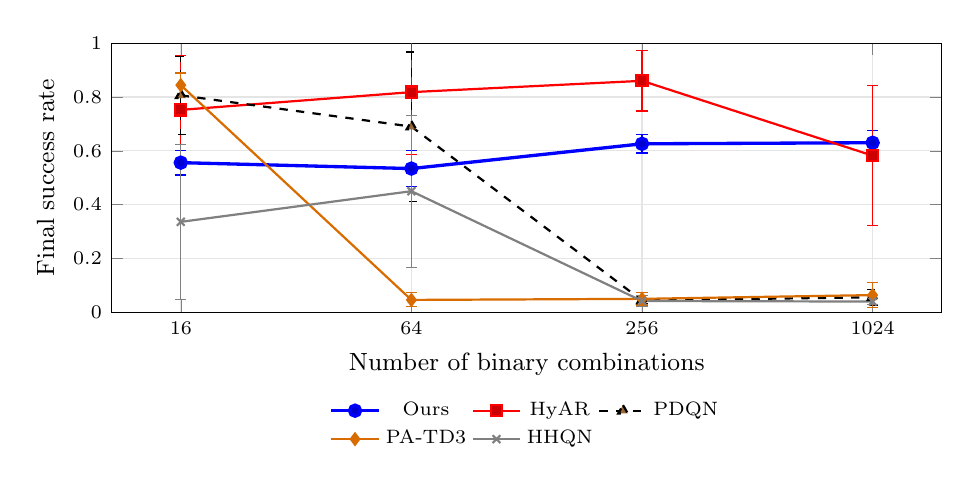
\begin{tikzpicture}
\begin{axis}[
    width=\columnwidth,
    height=5.0cm,
    ymin=0,
    ymax=1,
    xlabel={Number of binary combinations},
    ylabel={Final success rate},
    xtick={1,2,3,4},
    xticklabels={16,64,256,1024},
    grid=major,
    grid style={gray!20},
    tick label style={font=\scriptsize},
    label style={font=\small},
    legend style={
        font=\scriptsize,
        at={(0.5,-0.29)},
        anchor=north,
        legend columns=3,
        draw=none
    }
]

\addplot+[
    blue,
    very thick,
    mark=*,
    error bars/.cd,
    y dir=both,
    y explicit
] coordinates {
    (1,0.556) +- (0,0.046)
    (2,0.534) +- (0,0.066)
    (3,0.626) +- (0,0.034)
    (4,0.630) +- (0,0.044)
};
\addlegendentry{Ours}

\addplot+[
    red,
    thick,
    mark=square*,
    error bars/.cd,
    y dir=both,
    y explicit
] coordinates {
    (1,0.752) +- (0,0.203)
    (2,0.818) +- (0,0.232)
    (3,0.860) +- (0,0.112)
    (4,0.582) +- (0,0.259)
};
\addlegendentry{HyAR}

\addplot+[
    black,
    dashed,
    thick,
    mark=triangle*,
    error bars/.cd,
    y dir=both,
    y explicit
] coordinates {
    (1,0.806) +- (0,0.146)
    (2,0.690) +- (0,0.277)
    (3,0.044) +- (0,0.011)
    (4,0.056) +- (0,0.029)
};
\addlegendentry{PDQN}

\addplot+[
    orange!85!black,
    thick,
    mark=diamond*,
    error bars/.cd,
    y dir=both,
    y explicit
] coordinates {
    (1,0.844) +- (0,0.045)
    (2,0.046) +- (0,0.026)
    (3,0.050) +- (0,0.023)
    (4,0.064) +- (0,0.047)
};
\addlegendentry{PA-TD3}

\addplot+[
    gray,
    thick,
    mark=x,
    error bars/.cd,
    y dir=both,
    y explicit
] coordinates {
    (1,0.336) +- (0,0.288)
    (2,0.450) +- (0,0.282)
    (3,0.042) +- (0,0.019)
    (4,0.040) +- (0,0.010)
};
\addlegendentry{HHQN}

\end{axis}
\end{tikzpicture}
\caption{
Final HardMove success rate as the number of joint binary
configurations increases. The main comparison is the degradation
pattern as the action space grows from 16 to 1,024 combinations.
Error bars show sample standard deviations over five training seeds.
}
\label{fig:hardmove-success}
\end{figure}

제안 방법의 평균 성공률은 HM4부터 HM10까지 각각
$0.556$, $0.534$, $0.626$ 및 $0.630$이다. 즉 결합 행동 수가 16개에서 1,024개로 64배 증가했지만 관측된 성공률은 감소하지 않았으며, 평가범위에서 급격한 scaling collapse가 나타나지 않았다. HM10과 HM4의 평균차이로 본 성능 유지량은 제안 방법 $+0.074$, HyAR $-0.170$, PDQN $-0.750$, PA-TD3 $-0.780$, HHQN $-0.296$이다. 이 차이는 단일 크기에서의 순위와 별도로, 조합 수 증가에 따른 degradation을 직접 요약한다.

비교 방법의 절대 순위는 차원에 따라 달라진다. HyAR는 HM4--HM8에서 더 높은 평균을 기록한 뒤 HM10에서 $0.582$로 감소한다. PDQN과 PA-TD3는 HM4에서 각각 $0.806$과 $0.844$를 기록하지만 HM8--HM10에서는 $0.044$--$0.064$ 수준으로 낮아진다. 따라서 이 그림의 핵심 관찰은 모든 크기에서의 일률적인 우위가 아니라, 조합 수 증가에 대한 방법별 degradation 양상의 차이이다. HM10에서 제안 방법의 평균이 가장 높지만 방법 간 불확실성을 고려하여 통계적 우위로 해석하지 않는다. 모든 방법의 평균과 sample standard deviation은 Supplement에 제시한다.


\subsection{Performance--Cost Trade-off}

Fig.~\ref{fig:hardmove-runtime}은 제안 방법과 HyAR의 HardMove 평균 학습시간을 비교한다. HyAR는 잠재 행동표현과 디코더를 학습하는 반면 제안 방법은 실행 가능한 이진 행동의 가치구조를 직접 사용한다.

\begin{figure}[t]
\centering
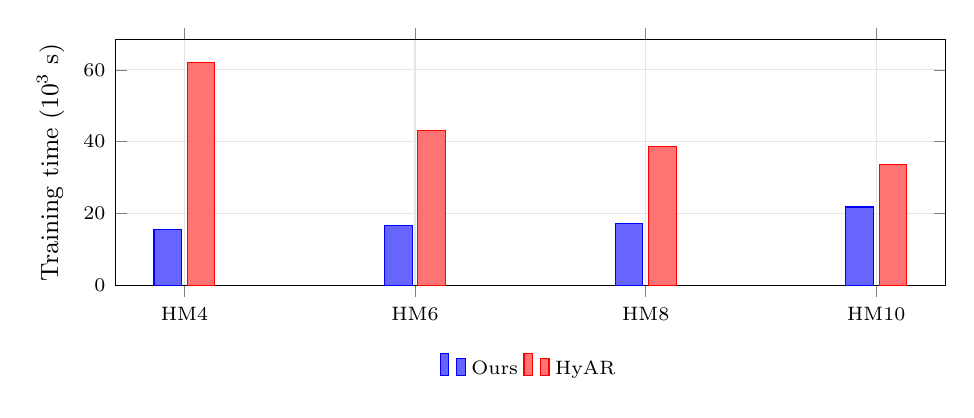
\begin{tikzpicture}
\begin{axis}[
    width=\columnwidth,
    height=4.7cm,
    ybar,
    bar width=10pt,
    ylabel={Training time ($10^3$ s)},
    symbolic x coords={HM4,HM6,HM8,HM10},
    xtick=data,
    ymin=0,
    grid=major,
    grid style={gray!20},
    tick label style={font=\scriptsize},
    label style={font=\small},
    legend style={
        font=\scriptsize,
        at={(0.5,-0.25)},
        anchor=north,
        legend columns=2,
        draw=none
    }
]

\addplot+[fill=blue!60] coordinates {
    (HM4,15.651)
    (HM6,16.681)
    (HM8,17.267)
    (HM10,21.807)
};
\addlegendentry{Ours}

\addplot+[fill=red!55] coordinates {
    (HM4,62.188)
    (HM6,43.160)
    (HM8,38.694)
    (HM10,33.612)
};
\addlegendentry{HyAR}

\end{axis}
\end{tikzpicture}
\caption{
Mean training time of the proposed method and HyAR on HardMove.
Runtime is reported together with the scaling curve to characterize
the performance--cost trade-off rather than to rank estimator kernels.
}
\label{fig:hardmove-runtime}
\end{figure}

제안 방법은 네 가지 HardMove 조건 모두에서 HyAR보다 짧은 평균 학습시간을 기록하였다. HM4에서는 제안 방법이 약 $15.7\times10^3$초, HyAR가 약 $62.2\times10^3$초를 사용하였다. HM10에서는 제안 방법이 약 $21.8\times10^3$초, HyAR가 약 $33.6\times10^3$초를 사용하여 제안 방법의 학습시간이 약 35\% 짧았다.

HM10에서 제안 방법은 $0.630$의 성공률과 약 $21.8\times10^3$초의 학습시간을 기록하고, HyAR는 $0.582$와 약 $33.6\times10^3$초를 기록하였다. 이 결과는 가장 큰 HardMove 조건에서 관측된 성능 유지가 더 긴 학습시간을 사용한 결과가 아님을 보여준다. 다만 각 구현의 전체 학습절차가 runtime에 포함되므로 이를 순수 estimator kernel의 속도 비교로 해석하지 않는다.


\subsection{Evaluation on Additional Environments}

Table~\ref{tab:cross-domain-results}은 HardMove와 다른 환경에서 제안 방법과 HyAR-TD3를 비교한 결과이다. Cogen-BC는 고정된 행동 설정에서의 적용성을 나타내며, GymInvMgmt-C6--C10은 다른 환경에서 행동 차원이 증가할 때의 성능 변화를 나타낸다. GymInvMgmt에서는 각 조건의 더 높은 평균 return을 굵게 표시하였다.

\begin{table}[t]
\centering
\caption{
Final return on additional environments over five training seeds.
Boldface marks the higher mean for the GymInvMgmt comparisons.
}
\label{tab:cross-domain-results}
\resizebox{\columnwidth}{!}{
\begin{tabular}{lcc}
\toprule
Environment & Ours & HyAR-TD3\\
\midrule
Cogen-BC
& $-3.927\mathrm{M}\pm0.352\mathrm{M}$
& $-32.471\mathrm{M}\pm14.677\mathrm{M}$\\

GymInvMgmt-C6
& $2015.5\pm33.2$
& $\mathbf{2029.0\pm73.6}$\\

GymInvMgmt-C8
& $1722.1\pm218.4$
& $\mathbf{1852.5\pm110.5}$\\

GymInvMgmt-C10
& $\mathbf{1562.3\pm227.5}$
& $1455.1\pm48.2$\\
\bottomrule
\end{tabular}
}
\end{table}

Cogen-BC의 고정된 6-bit 설정은 서로 다른 구조의 하이브리드 에너지 제어환경에 전체 프레임워크를 적용할 수 있는지를 확인하는 보조 결과이다. 이 조건에서는 제안 방법에 환경별 observation 및 Q normalization이 사용되므로, 방법 간 return 차이를 제안한 estimator 단독의 효과로 귀속하지 않는다.

GymInvMgmt-C6와 C8에서는 HyAR가 각각 $2029.0$과
$1852.5$의 평균 return을 기록하였다. 이진 행동 차원이 가장 큰 C10에서는 제안 방법이 $1562.3$의 평균 return으로 HyAR의
$1455.1$보다 높은 평균을 기록하였다. 절대 순위가 차원에 따라 바뀌므로 이 결과는 전 구간 우위가 아니라, HardMove와 다른 재고관리 환경의 가장 큰 평가조건에서도 제안 방법의 성능이 급락하지 않았다는 보조 증거로 사용한다.

계산비용 측면에서 제안 방법의 평균 행동 생성 지연은 약 $0.317$ ms이고 HyAR는 $0.843$ ms이다. 제안 방법은 HyAR보다 약 62\% 짧은 행동 생성 지연을 기록하였다. 평균 환경 처리량도 제안 방법이 $76.8$ step/s, HyAR가 $72.6$ step/s로 측정되었다.

GymInvMgmt에서는 C6와 C8에서 HyAR의 평균이 높고 C10에서 제안 방법의 평균이 높아, 환경과 차원에 따라 절대 순위가 달라진다. 동시에 제안 방법의 더 짧은 행동 생성 지연은 잠재 행동 디코딩 없이 연속 행동과 이진 행동을 직접 생성하는 구조의 실행비용 특성을 보여준다.


\subsection{Component Ablation}

핵심 구성요소의 효과는 가장 큰 HardMove 조건인 HM10에서 평가한다. Ablation은 동일한 1M interaction budget과 다섯 개의 training seed를 사용한 별도의 실험군으로 수행한다. Table~\ref{tab:hm10-ablation}은 전체 방법과 각 구성요소를 제거하거나 대체한 변형의 성공률을 비교한다.

\begin{table}[t]
\centering
\caption{
Component ablation on HardMove-10.
Results are mean and sample standard deviation over five seeds.
The ablation uses an independently sampled set of training seeds.
}
\label{tab:hm10-ablation}
\resizebox{\columnwidth}{!}{
\begin{tabular}{lcc}
\toprule
Variant & Success rate & Runtime (s)\\
\midrule
Full method
& $\mathbf{0.642\pm0.048}$
& 19,418\\

Marginal-logit policy (without $J$)
& $0.632\pm0.033$
& 24,987\\

Unary critic/surrogate (without pair terms)
& $0.540\pm0.213$
& 21,998\\

Random MC design (same row budget)
& $0.634\pm0.043$
& 22,842\\

Plain IS (without ACV correction)
& $0.430\pm0.261$
& 19,061\\

Independent binary policy
& $0.198\pm0.337$
& 14,428\\
\bottomrule
\end{tabular}
}
\end{table}

전체 방법은 $0.642$의 평균 성공률을 기록하였다. $J$를 제거하여 상태별 marginal logits만 사용하는 변형과의 평균차이는 0.010으로 작았다. 이는 $J$가 필수적인 확률상관 모형이라기보다 이 구현에서 이진 평균을 조정하는 보조 모듈임을 보여준다. Pair terms를 제거하되 동일한 native actor를 유지한 unary critic/surrogate 변형과의 평균차이는 0.102였으나, 후자의 seed 변동성은 컸다.

동일한 row budget에서 조건수 제약 설계를 무작위 Monte Carlo 질의로 대체한 변형은 유사한 평균 성공률을 기록하였고, 전체 방법의 평균 실행시간은 3,424초 짧았다. 따라서 이 비교는 질의설계의 보편적인 정책성능 우위보다 해당 구현에서의 계산효율 차이를 보여준다. ACV correction을 제거한 변형은 동일한 native actor와 중요도 표본을 유지하되 plain importance-sampled score gradient를 사용한다. 전체 방법의 평균은 이 변형보다 0.212 높았지만, 두 실험군의 분산을 고려하여 estimator 하나의 보편적 우위로 일반화하지 않는다.

Independent 정책과 비교하면 전체 방법의 평균 성공률은 0.444 높았다. 이 ablation의 일관된 해석은 HM10에서 결합 행동구조와 잔차 보정을 함께 유지한 구성이 더 높은 평균을 기록했다는 것이다. 개별 구성요소의 독립적인 효과나 다른 환경으로의 일반화는 seed 변동성을 고려하여 별도로 확정하지 않는다.


\section{Discussion}
\label{sec:discussion}

실험결과는 조합공간이 커질 때 나타나는 성능과 비용의 변화를 중심으로 해석한다. HardMove의 통제된 차원 증가, GymInvMgmt의 교차환경 차원 증가 및 runtime 측정은 각각 성능 유지 양상, 적용범위 및 계산특성을 서로 다른 관점에서 평가한다. 다음 절에서는 이 관찰을 학습--실행 일관성, 구성요소 및 계산복잡도와 연결한다.

\subsection{Consistency between Learning and Execution}

제안 방법의 핵심은 환경에서 실행되는 이진 행동과 정책 갱신에 사용되는 연속 변수 사이의 가치관계를 명시적으로 정의하는 데 있다. 크리틱은 replay buffer에 저장된 실제 이진 행동으로 학습되며, 이완된 스핀 $S$에서의 가치는 해당 크리틱의 Bernoulli 다중선형 기대값으로 계산된다. 따라서 정책이 사용하는 연속 가치표현은 별도의 이완 크리틱에 의해 결정되지 않고 실행 가능한 이진 행동의 가치로부터 직접 구성된다.

내부점에서 다중선형 목적은 $\mu_S$에 따른 확률적 학습정책의 기대가치인 반면, 평가정책은 $\operatorname{sign}(S)$로 결정론적이다. 두 목적은 일반적으로 동일하지 않으며 $S$가 꼭짓점에 가까워질 때 일치한다. 본 연구는 binary regularization으로 내부점과 꼭짓점의 차이를 줄인다. 따라서 꼭짓점 일치성은 모든 학습 단계의 평가정책 일치를 의미하는 것이 아니라, 이완이 꼭짓점에 접근할 때의 일치 조건을 제공한다.

구체적으로 이진 학습목적과 평가목적은 각각
\begin{align}
J_{\mathrm{train}}(S)
&=\E_{Z\sim\mu_S}
[Q_{\min}^{\mathrm{hard}}(s,a^c,Z)],\\
J_{\mathrm{eval}}(S)
&=Q_{\min}^{\mathrm{hard}}
(s,a^c,\operatorname{sign}(S))
\end{align}
이다. 제안된 score estimator는 고정된 learned critic에 대한 $\nabla_SJ_{\mathrm{train}}$의 불편 추정량이다. 환경 return의 기울기나 결정론적 $J_{\mathrm{eval}}$의 불편 추정량을 제공하는 것은 아니다. Binary regularization은 두 목적의 차이를 줄이도록 유도하지만 이를 완전히 제거하지는 않는다.

연속 행동과 이진 행동은 동일한 hard-action critic을 사용하지만 서로 다른 gradient 경로로 최적화된다. 연속 행동은 결정론적 평가 이진 행동에서 critic의 행동 미분을 사용하고, 이진 정책은 mixture proposal에서 얻은 중요도 가중 ACV score gradient를 사용한다.


\subsection{Interpretation of the Structured Estimator}

정확한 black-box 다중선형 합은 $2^b$개의 이진 행동 조합을 포함한다. 본 구현은 정책기울기를 해석적으로 계산되는 ANOVA 성분과 표본으로 추정되는 amortization 잔차 성분으로 분리하여 질의 수가 전체 조합 수를 따라 증가하지 않도록 한다.

ANOVA 대리모형의 기대값은
$\E[z_i]=S_i$와 $\E[z_iz_j]=S_iS_j$를 이용하여 추가적인 크리틱 질의 없이 계산할 수 있다. 이는 반복적인 정책 갱신에서 동일한 저차 가치구조를 표본으로 다시 추정하는 비용을 줄인다. 행동 간 상호작용은 선택된 쌍 $(i,j)\in\mathcal{E}$에 대응하는 $S_iS_j$ 항으로 정책 기울기에 직접 반영된다.

ANOVA network는 최종 가치함수가 아니라 제한된 질의에서 반복되는 저차 구조를 재사용하는 제어변량으로 사용된다. 대리모형과 hard-action critic의 차이는 중요도 가중 score 항으로 보정되므로, 이진 정책기울기는 amortized 계수의 근사오차만으로 결정되지 않는다. 여기서 핵심적인 시스템 수준의 역할은 특정 추정기의 순위를 정하는 것이 아니라, 결합 상호작용을 유지하면서 $2^b$개의 직접 평가를 피하는 데 있다.

조건수 검사는 선택된 주효과와 쌍대 항이 질의값에서 식별 가능한지를 확인하는 구현 장치이다. 동일 row budget의 Monte Carlo 질의와 HM10 평균 성공률이 유사하므로 이를 별도의 정책성능 기여로 해석하지 않는다.


\subsection{Contribution of the Main Components}

HM10 ablation에서 잔차 보정을 제거한 변형은 $0.430$의 평균 성공률을, 전체 구성은 $0.642$를 기록하였다. 이 비교는 제한된 질의에서 대리모형만 사용하는 것보다 잔차까지 반영한 구성이 해당 실험군에서 더 안정적인 평균을 보였음을 나타낸다. 제거 변형의 seed 변동성이 크므로 차이는 전체 구성의 동작을 이해하는 근거로 사용한다.

쌍대 항을 제거한 변형은 $0.540$의 평균 성공률을 기록하였다. 전체 방법과의 평균차이는 행동쌍 상호작용이 HM10에서 유용할 가능성을 지지하지만, 이 변형 역시 seed 변동성이 크므로 그 독립적 효과를 확정하지 않는다.

Independent 정책의 평균 성공률은 $0.198$로 전체 방법보다 0.444 낮았다. 이 결과는 평가한 HM10 설정에서 결합 가치구조를 사용하는 전체 구성이 독립 정책보다 높은 평균을 기록했음을 보여주며, 개별 모듈 하나의 효과로 귀속하지 않는다.

$J$를 제거한 marginal-logit 변형의 평균은 전체 방법과 유사하였다. 실제 표본은 $J$의 유무와 관계없이 product Bernoulli이므로, $J$는 상관된 sampler가 아니라 상태 조건부 logit adjustment이다. HM10의 주된 구성 근거는 pairwise value representation과 residual-corrected update에서 나타난다.


\subsection{Scaling Behavior across Environments}

HardMove 실험은 동일한 환경구조에서 이진 행동 차원만 변화시킨다. 가능한 이진 조합 수가 16개에서 1,024개로 증가하는 동안 제안 방법의 평균 성공률은 $0.534$--$0.630$ 범위였고, HM10 학습시간은 HyAR보다 약 35\% 짧았다. HM4--HM8에서는 HyAR의 평균 성공률이 더 높고 HM10의 방법 간 차이는 seed 변동성에 비해 작다. 따라서 이 결과의 핵심은 전 구간의 순위가 아니라, 평가범위에서 제안 방법이 추가 계산시간에 의존하지 않으면서 급격한 성능 붕괴를 보이지 않았다는 점이다.

GymInvMgmt는 HardMove와 다른 상태전이와 보상구조에서 이진 행동 차원을 6, 8, 10으로 증가시킨다. 가장 큰 C10 조건에서 제안 방법은 HyAR보다 높은 평균 return을 기록하였다. 또한 제안 방법의 행동 생성 지연은 $0.317$ ms로 HyAR의 $0.843$ ms보다 짧았다. 정책이 잠재 행동을 별도로 복원하지 않고 이진 행동과 연속 행동을 직접 생성하는 구조는 실행 단계의 계산비용을 줄인다.

Cogen-BC의 고정된 6-bit 결과는 scaling curve가 아니라 다른 행동 의미와 보상구조에서의 적용성을 보완한다.


\subsection{Computational Characteristics}

정확한 black-box 다중선형 합의 질의 수는 $O(2^b)$이지만, 제안 방법의 정책 갱신 질의점 수는 설계질의 $N_{\mathrm{des}}$와 잔차 표본 $M$의 합으로 결정된다. 희소 ANOVA에서 $K$개의 쌍만 선택하면 대리모형의 항 수와 해석적 기대값 계산량은 $O(b+K)$가 된다. 이 결과는 estimator의 query budget에 관한 것이며 전체 actor--critic update의 선형 복잡도를 의미하지 않는다.

이 구조는 결합 행동 수 전체가 아니라 선택된 상호작용과 질의 예산에 따라 계산량을 조절할 수 있게 한다. 정책 네트워크는 $b$개의 이진 제어변수를 출력하고, 가치추정기는 사전에 정한 예산 안에서 hard critic을 질의한다. 따라서 이진 차원이 증가하더라도 정책 또는 크리틱이 $2^b$개의 출력을 직접 생성할 필요가 없다.

계산 효율은 학습뿐 아니라 실행 단계에서도 나타난다. 학습 시에는 구조화된 대리모형과 잔차 표본을 사용하여 전체 행동 열거를 피한다. 실행 시에는 학습된 액터와 스핀 모듈을 한 번 평가하고 성분별 부호함수를 적용하여 이진 행동을 생성한다. 별도의 후보 행동검색이나 잠재 행동 디코딩이 필요하지 않으므로 행동 생성비용이 결합 행동 수 $2^b$에 대해 지수적으로 증가하지 않는다. 다만 $J_\psi(s)$를 명시적으로 생성하는 현재 구현의 비용은 $b$에 대해 $O(b^2)$이다.


\section{Limitations and Future Work}
\label{sec:limitations}

현재 방법은 MultiBinary 행동과 주효과--쌍대 상호작용을 대상으로 한다. 따라서 MultiCategorical 행동이나 강한 고차 상호작용에는 직접 적용되지 않는다. 범주형 simplex를 이용한 확장과 고차 critic은 가능한 후속 방향이다.

$N_{\mathrm{des}}$, $K$ 및 $M$은 현재 사전에 정하며, policy-learning 평가는 최대 $b=10$으로 제한된다. 더 큰 공간에서는 importance-weight concentration과 interaction selection을 함께 측정하고, 상태별 잔차와 entropy에 따라 질의예산을 조정할 필요가 있다.

이론은 고정된 critic에 대한 꼭짓점 일치성, 조건부 가치차 및 score-gradient 불편성을 다루며 환경 return의 최적화나 수렴을 보장하지 않는다. 유한질의 오차경계와 정책개선량의 관계는 향후 분석과제로 남는다.


\section{Conclusion}
\label{sec:conclusion}

본 연구는 결합 행동 수가 지수적으로 증가하는 이진--연속 행동공간을 위해 native hybrid-action actor--critic을 제안하였다. 정책은 전체 조합을 범주형으로 열거하지 않고 연속 행동과 복수의 이진 행동을 직접 생성하며, executed-action twin critic은 pairwise value structure를 표현한다. Residual-corrected multilinear update는 개별 critic 기대값의 최솟값으로 목적을 바꾸지 않고, 실제 clipped-twin objective를 제한된 hard-action 질의로 정책학습에 전달한다.

HardMove에서 이진 조합 수가 16개에서 1,024개로 증가하는 동안 제안 방법의 평균 성공률은 급격히 감소하지 않았다. 비교 방법의 순위는 차원에 따라 달라졌지만, 여러 범주형 또는 파라미터화 기준선에서 나타난 큰 성능저하가 제안 방법에서는 관찰되지 않았다. 동시에 HM10의 평균 학습시간은 HyAR보다 약 35\% 짧았으며, 직접적인 행동생성 구조는 추가 환경에서도 더 짧은 action latency를 기록하였다.

추가 환경의 결과는 이 관찰을 서로 다른 전이 및 보상구조에서 보완한다. Ablation은 pairwise value representation과 residual correction을 함께 유지한 전체 구성이 HM10에서 안정적인 평균을 기록했음을 보여준다. 종합하면 제안 구조는 평가한 범위에서 조합공간 증가에 따른 성능 붕괴와 계산비용 증가를 함께 완화하는 일관된 특성을 보였다.


\begin{thebibliography}{99}

\bibitem{yeh2023}
C. Yeh, V. Li, R. Datta, J. Arroyo, N. Christianson,
C. Zhang, Y. Chen, M. M. Hosseini, A. Golmohammadi,
Y. Shi, Y. Yue, and A. Wierman,
``SustainGym: Reinforcement learning environments
for sustainable energy systems,''
in \emph{Advances in Neural Information Processing Systems},
vol. 36, 2023,
doi: 10.52202/075280-2598.

\bibitem{masson2016}
W. Masson, P. Ranchod, and G. Konidaris,
``Reinforcement learning with parameterized actions,''
in \emph{Proc. AAAI Conf. Artif. Intell.},
vol. 30, no. 1, pp. 1934--1940, 2016,
doi: 10.1609/aaai.v30i1.10226.

\bibitem{xiong2018}
J. Xiong, Q. Wang, Z. Yang, P. Sun, L. Han, Y. Zheng,
H. Fu, T. Zhang, J. Liu, and H. Liu,
``Parametrized deep Q-networks learning:
Reinforcement learning with discrete-continuous hybrid action space,''
\emph{arXiv preprint arXiv:1810.06394}, 2018,
doi: 10.48550/arXiv.1810.06394.

\bibitem{bester2019}
C. J. Bester, S. D. James, and G. D. Konidaris,
``Multi-pass Q-networks for deep reinforcement learning
with parameterised action spaces,''
\emph{arXiv preprint arXiv:1905.04388}, 2019,
doi: 10.48550/arXiv.1905.04388.

\bibitem{fan2019}
Z. Fan, R. Su, W. Zhang, and Y. Yu,
``Hybrid actor-critic reinforcement learning
in parameterized action space,''
in \emph{Proc. 28th Int. Joint Conf. Artif. Intell.},
pp. 2279--2285, 2019,
doi: 10.24963/ijcai.2019/316.

\bibitem{li2022hyar}
B. Li, H. Tang, Y. Zheng, J. Hao, P. Li, Z. Wang,
Z. Meng, and L. Wang,
``HyAR: Addressing discrete-continuous action reinforcement
learning via hybrid action representation,''
in \emph{Proc. Int. Conf. Learn. Representations}, 2022.

\bibitem{dulacarnold2015}
G. Dulac-Arnold, R. Evans, H. van Hasselt, P. Sunehag,
T. Lillicrap, J. Hunt, T. Mann, T. Weber, T. Degris,
and B. Coppin,
``Deep reinforcement learning in large discrete action spaces,''
\emph{arXiv preprint arXiv:1512.07679}, 2015,
doi: 10.48550/arXiv.1512.07679.

\bibitem{tavakoli2018}
A. Tavakoli, F. Pardo, and P. Kormushev,
``Action branching architectures for deep reinforcement learning,''
in \emph{Proc. AAAI Conf. Artif. Intell.},
vol. 32, no. 1, pp. 4131--4138, 2018,
doi: 10.1609/aaai.v32i1.11798.

\bibitem{lee2025}
J. Lee, T. Gao, E. Nelson, M. Liu, D. Bhattacharjya,
and S. Lu,
``Q-function decomposition with intervention semantics
for factored action spaces,''
in \emph{Proc. 28th Int. Conf. Artif. Intell. Statist.},
ser. Proc. Mach. Learn. Res., vol. 258, pp. 1027--1035, 2025.

\bibitem{jang2017}
E. Jang, S. Gu, and B. Poole,
``Categorical reparameterization with Gumbel-Softmax,''
in \emph{Proc. Int. Conf. Learn. Representations}, 2017.

\bibitem{maddison2017}
C. J. Maddison, A. Mnih, and Y. W. Teh,
``The Concrete distribution:
A continuous relaxation of discrete random variables,''
in \emph{Proc. Int. Conf. Learn. Representations}, 2017.

\bibitem{calinescu2011}
G. Calinescu, C. Chekuri, M. P{\'a}l, and J. Vondr{\'a}k,
``Maximizing a monotone submodular function subject to
a matroid constraint,''
\emph{SIAM J. Comput.},
vol. 40, no. 6, pp. 1740--1766, 2011,
doi: 10.1137/080733991.

\bibitem{owen1992}
A. B. Owen,
``Orthogonal arrays for computer experiments,
integration and visualization,''
\emph{Statistica Sinica},
vol. 2, no. 2, pp. 439--452, 1992.

\bibitem{owen1994}
A. B. Owen,
``Lattice sampling revisited:
Monte Carlo variance of means over randomized orthogonal arrays,''
\emph{Ann. Statist.},
vol. 22, no. 2, pp. 930--945, 1994,
doi: 10.1214/aos/1176325509.

\bibitem{tracey2016}
B. D. Tracey and D. H. Wolpert,
``Reducing the error of Monte Carlo algorithms
by learning control variates,''
\emph{arXiv preprint arXiv:1606.02261}, 2016,
doi: 10.48550/arXiv.1606.02261.

\bibitem{fujimoto2018}
S. Fujimoto, H. van Hoof, and D. Meger,
``Addressing function approximation error
in actor-critic methods,''
in \emph{Proc. 35th Int. Conf. Mach. Learn.},
vol. 80, pp. 1587--1596, 2018.

\end{thebibliography}

\end{document}
